\section{Language Choose}
\subsection{JavaScript’s  features}	\cite{7}
\\
Node.js is based on JavaScript design \\
\\
JavaScript is a scripting language that based on the object and event driven, and it also good at security capability, JavaScript is dedicated to develop INTERNET client and server applications, it can be embedded into HTML file easily, and through the built-in interpreter of the JavaScript in the browser to perform. Using JavaScript, the browser can respond to the needs of users events without back data through the network. In this way, the user's data can be directly by the client application processing. It also can easily realize the interaction with network customers, and make the web becomes vivid.\\
\\
Forexample: when you visit a website, JavaScript can give responses immediately by move mouse or click some button or other component in this page or drag windows and etc.\\
\\
\subsection{Object-Oriented}
\\
Talking about the object-oriented programming language, most people immediately think of C++ and Java that a strongly typed language, Python, and Ruby, scripting languages, their common feature is a class-based object-oriented. And when it comes to JavaScript, it's hard to make people think its object-oriented programing language, because it does not have any classes. Although JavaScript does not have classes, but JavaScript is an object-oriented language. JavaScript object only, and an object is object, not an instance of the class. Because most are based on class of objects in object-oriented languages, it is easy to misunderstand the concepts of an instance of the class with the object. The definition of object is an instance of the class maybe correct in most other languages, but it’s not for JavaScript.\\ 
\\
\subsection{Variable and Object} 
\\
The object in JavaScript actually is a related Array that made by property which consisted by name and value, the value type can be any data type, or a function, and other objects. JavaScript has a special characteristic of functional programming, so function also is a variable, most of the time same as general data types. In JavaScript, use the dot operator is equal with an associative array reference, meaning that any object (including the this pointer) can use either mode. Are the benefits of using an associative array, if in a case but you do not know the names of the object, you can use an index as an associative array.\\ 
\\
\subsection{Cross-Platform}
\\
JavaScript scripting language is not dependent on the operating system, only need the support of the browser. So JavaScript can be used to any machine, after writing the premise on the machine on browsers support JavaScript scripting language, JavaScript is supported by most browsers.\\
\\
\section{Node.js}\cite{1}
\\
Use Node.js with MongoDB to develop this website because human being already come in Big Data, huge amount data need processing through browser. So the efficiency especially important in a web application, and now Node.js can provide a high-efficiency platform to develop web.\\
\\
\subsection{ Node.js's advantages on web development}
\\
Node.js use event-driven, asynchronous programming, and network design services. In fact, anonymous functions and closures characteristics JavaScript is ideal for event-driven, asynchronous programming. And JavaScript are easy to learn, a lot of front-end designers can quickly get started doing back-end design.\\
\\
Node.js non-blocking mode processing to bring in relatively low system resource consumption at high performance and outstanding load capacity, very suitable for mid-tier service used to rely on other IO resources. And Node.js lightweight and efficient, it can be considered the perfect solution for data-intensive real-time applications distributed deployment environment under. Node is very suitable for the following: In response to a client before, you may be expected to have a high traffic, but the required server-side logic and processing is not necessarily a lot.\\
\\
\subsection{Powerful Institutions are used Node.js}
\\	
1.Pay Pal \cite{5}\\
There have a paper was written by Jeff Harrell show the sharp increasing of efficiency, amount of code and performance after PayPal use Node.js to develop application.\\
There have a competition in PayPal engineers, one team with five engineers working on java application, another team with two people working on Node.js application and they are need to realize same functions. In the end, when they ran the test cases ,the node.js app was:\\
•	Built almost twice as fast with fewer people\\
•	Written in 33\% fewer lines of code\\
•	Constructed with 40\% fewer files\\
\\
2.Twitter queue\\
Imagine companies such as Twitter, it must receive tweets and written to the database. In fact, almost every second thousands tweet reached, the database cannot be processed in time to write the huge number of message in peak hours. Node.js has become an important part of the problem solution. As you can see, Node can handle tens of thousands of tweet. It can write them to a memory queuing mechanism (such as mecached) quickly and easily, a separate process will written those tweet to the database. Node's role here is to quickly collect tweet, and this information is passed to the process and the other for writing. Imagine another design (regular PHP server will attempt to process its own writes to the database itself): Each tweet will lead to a short delay when writing to the database because the database call blocking passage. Since the database delay, machine could only handle 2000 incoming tweet every second. 1 million per second tweet need 500 servers. Instead, Node can handle each connection without blocking the passage, it is possible to capture as many tweets. A tweet can handle 50,000 machines in just 20 of Node server.
\\
\section{Architecture Review(uml)} 
\subsection{system Architecture(uml)} 
I used a minimal and flexible Framework to make my website is Express.js, and there also have some functions it need have and show those below:\\
\\
(1) Route maps.\\
Different types of requests can be mapped to different business logic, which should include requests for static data and data requests for the distribution.\\
(2) The Cookie feature.\\
 Meet the needs of certain data need to be stored in the client browser.\\
(3)Session function.\\
Realize Session conversation by Cookie, and to store a small amount of data throughout the session.\\
(4) Property injection function. \\
Use JavaScript to parse the form data and put into the appropriate business logic implementations.\\
(5) The dynamic method invocation:\\
 URL calls according to the rules in the same business logic object in the specified method.\\
\\
Key processes are:\\
1.	Client sends a request to the server, services send the client’s request to the Filter.\\ 
2.	Through analysis, filter and process of the requested data, and then passes the request to the next level of routing the dispenser.\\
3.	 Routing the dispenser according to the related configuration to determine the requested property is a business data or static resource request, pass to appropriate handlers.\\
4.	 If read as a static resource then requests a static resource returned to the client.\\ 
5.	If business data request, depending on routing rules for forwarding to the appropriate business logic processing.\\
6.	 When processing is complete turn the data into JSON format back to the client.\\
\\
see graph \ref{fig:2 cubed graph} below:
\begin{figure}[h]
	\centering
	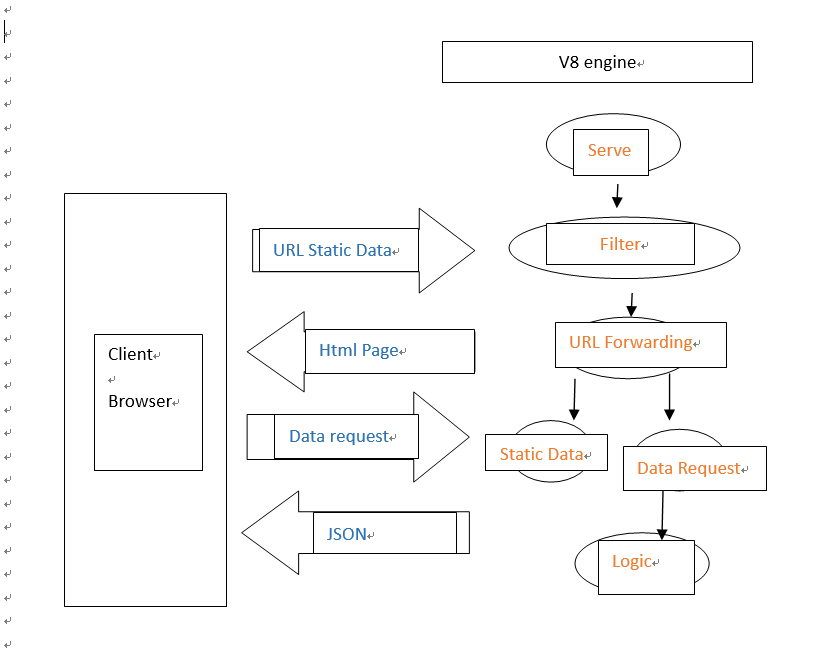
\includegraphics[scale=0.5]{27.png}
	\caption{Key processing}
	\label{fig:2 cubed graph}
\end{figure}
\\
\section{System Functions Review(uml)}
According to the functional requirements of the system, online shopping system is divided into the front-end management and back-end management. Front-end management, including browsing, query items, order merchandise, shopping carts, user information maintenance functions. Back-end management includes order management, items management, and user management module.\\
\\
Front-end is described as follows:\\
\\
1. Browse products\\
   Product details\\
   Item id\\
\\
 2 . Search for commodity\\
   Product category\\
   Product keyword\\
   Order inquiries\\
   \\
3. Order Item\\
\\
4. Shopping cart\\
\\
5. Users information maintenance\\
   User registration\\
   User login\\
   Modify user information\\
   \\
   ~      ~         ~               ~
Back-end and described as follows:\\
\\
1. Products management\\
  Add a product category\\
  Modify the product category\\
  Delete product categories\\
  Adding product information, including product category, name, number, company and other information;\\
  Product image upload, modify, and delete;\\
  Modify product information\\
  Delete product information\\
  View product information\\
  \\
2. Order management\\
  Processing orders\\
  Handling shipments\\
  Checks out\\
  Delete orders\\ 
\\
3. Complaint management\\
  Into complaints solutions\\
  Delete a resolved complaints\\
  View complaint support\\
  \\
4. Customer support management\\
  Registered customer, including the user name, password and other information\\
  Modify the customer information\\
  Delete the customer information\\
  \\
5. User management functions of the system\\
\\
  Add system users, including user name, password and other information;\\
  Modify user information systems;\\
  Delete system user information.\\
\\
And show a graph of those connection below graph \ref{fig:3 cubed graph}\\
\begin{figure}[h]
	\centering
	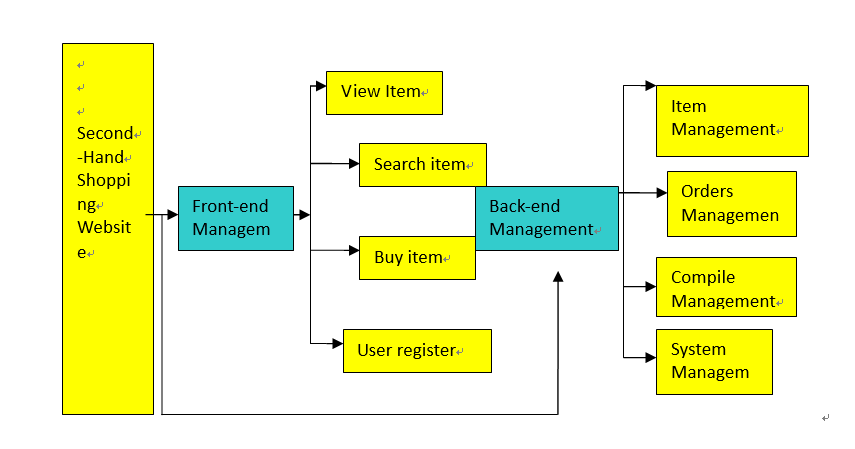
\includegraphics[scale=0.5]{28.png}
	\caption{Website Function modular}
	\label{fig:3 cubed graph}
\end{figure}
\\
Functions on Shopping website\\
 \\
	In this System, user Management module is pretty simply. In this system have a default user is admin (username: Admin, Password: Admin) which can add consumer user to Database and do some operation such as delect, update and create. And Normal consumers user only can manage them own account modify name and password, and change items that post by themselves.\\
	\\
And show graph below graph \ref{fig:4 cubed graph}:
\\
\begin{figure}[h]
	\centering
	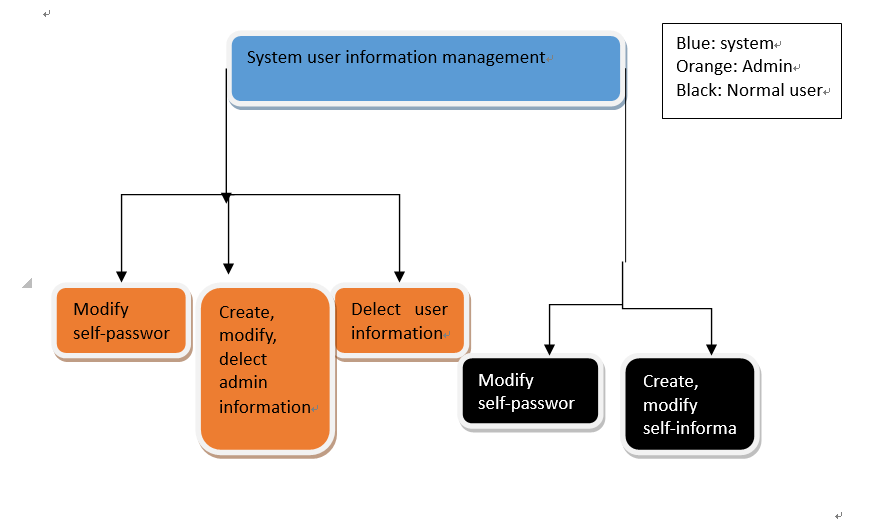
\includegraphics[scale=0.5]{29.png}
	\caption{User Management}
	\label{fig:4 cubed graph}
\end{figure}
\\
Normal Consumer shopping Steps show below graph \ref{fig:5 cubed graph}:\\
\\
\begin{figure}[h]
	\centering
	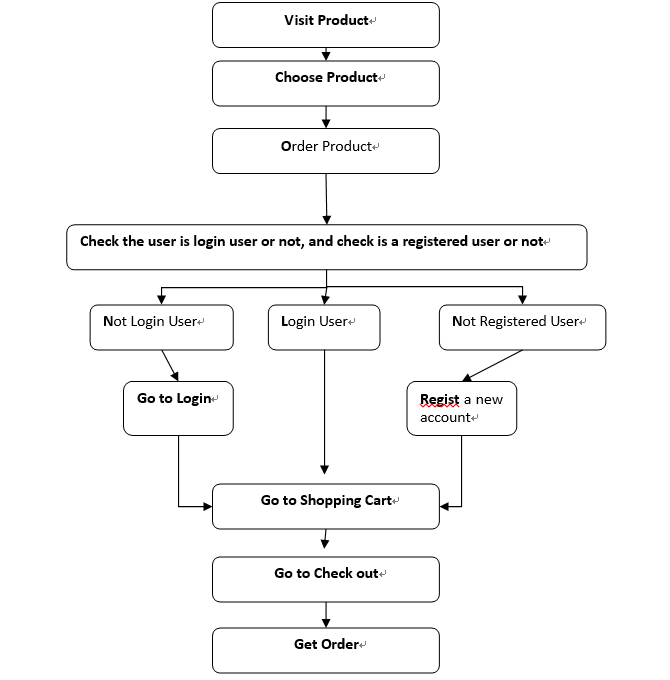
\includegraphics[scale=0.5]{30.png}
	\caption{Normal User Shopping Steps}
	\label{fig:5 cubed graph}
\end{figure}
  \\
\section{Security System}
There have some special design I did for built a prefect security system.
\subsection{Consumer's Password}
	When user register a new account, back-end will check this value of password.\\
 (1)	Check then length of password see graph \ref{fig:a cubed graph}:\\
 \begin{figure}
 	\centering
	 \begin{subfigure}[h]{0.3\textwidth}
	 	\centering
	 	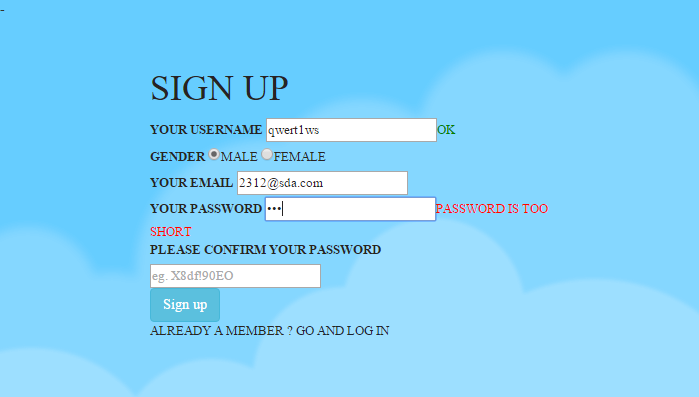
\includegraphics[width=\textwidth]{15.png}
	 	\caption{Register page}
	 	\label{fig:a cubed graph}
	 \end{subfigure}
 	\hfill
	 \begin{subfigure}[h]{0.3\textwidth}
	 	\centering
	 	
\includegraphics[width=\textwidth]{16.png}
	 	\caption{Password Check}
	 	\label{fig:c cubed graph}
	 \end{subfigure}	
 	\hfill
	 	\begin{subfigure}[h]{0.3\textwidth}
	 		\centering
	 		
\includegraphics[width=\textwidth]{17.png}
	 		\caption{Password Check}
	 		\label{fig:d cubed graph}
	 	\end{subfigure}
 	\caption{Register page Password Check}
 	\label{fig:ss graphs}
 \end{figure}
 
 (2) When user click sign up back-end will convert consumers' password to a log string use Crypto modular. The algorithm it used is AES-128-ECB, and then use BASE64 to encoding. It make sure user's information will store in server-end safety. The graph \ref{fig:7 cubed graph} show below is encrypted password:\\
 \\
 \begin{figure}[h]
 	\centering
 	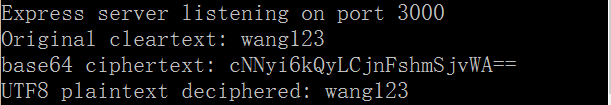
\includegraphics[scale=0.5]{18.png}
 	\caption{Encryption}
 	\label{fig:7 cubed graph}
 \end{figure}
 \\
\subsection{Session and Cookies}\cite{session}
\\
Cookies, session are method used to store user state information.
The main difference is:\\
(1) location: cookies are stored on the client side, the session on the server\\
(2) Security: cookies, poor safety, the session high safety\\
(3) life cycle: in the case of not set conditions both disappeared in the browser is turned off\\
(can be setting cookies on the client survival time, also can be installed on the server session time of survival)\\
Two relations, the session is implemented through a cookie
\\
So, in my final project I choose use session to store the most data rather then use cookies
\\
\subsection{Database Security Design}
\\
In MongoDB 2.4 version it do a new adjustment on users right management, refine the permissions, enhanced security.
So in this Project I also use Auth function create many different account to control different Database.
If use an unauthorized account to login database, It’s not allow to access into and can’t get any data from database, and protect users and items information from server-end.
\\
Open auth function\\
mongod --dbpath (db address) --port 27017  --logpath (mongodb.log address) --logappend --auth
\\
Images \ref{fig:8 cubed graph}\&\ref{fig:9 cubed graph} below is show the user and how it work:
If use unauthorized account login
 \\
 \begin{figure}[h]
 	\centering
 	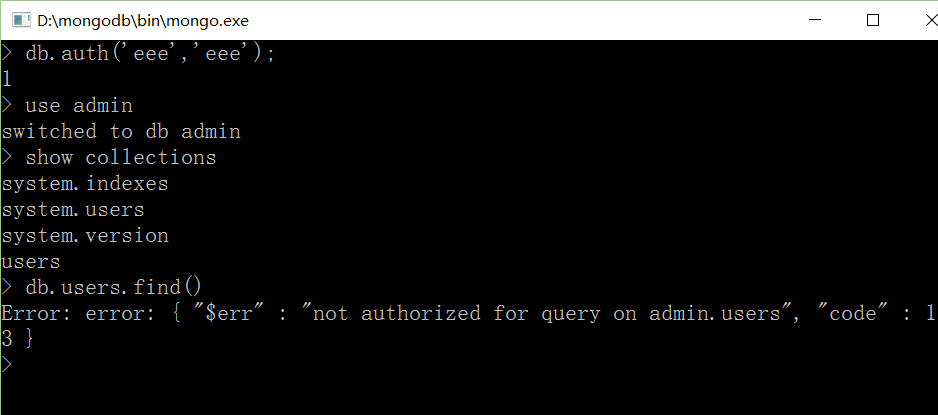
\includegraphics[scale=0.5]{19.png}
 	\caption{Database account}
 	\label{fig:8 cubed graph}
 \end{figure}
 
\begin{figure}[h]
	\centering
	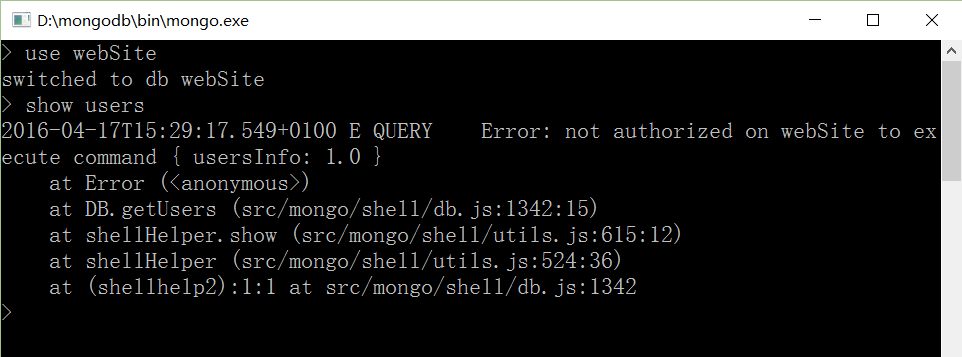
\includegraphics[scale=0.5]{20.png}
	\caption{Reject access}
	\label{fig:9 cubed graph}
\end{figure}
 \\
\subsection{Face to Face Trade}
If consumer want to buy something from Second-Hand shopping website, they can use city-wide search get the seller’s contact method such as email or phone number or Facebook and trade face to face.\\
Because consumers can’t see the real situation of this product when they are shopping online. So, if they can trade with seller face to face they can check the product first and thinking buy or not.\\
\\
\section{Database design}
In this project, I use MongoDB to store, update and delect user and item information.\\
\\
\subsection{Database Users}
All users in Database is in table \ref{tab:3} below :\\
\begin{table}[h]
	\centering
	\begin{tabular}{l | l| l| l}
		Database & Username & Password& Role \\
		\hline
		Admin & Harry & Harry & userAdminAnyDatabase \\
		Admin & admin & admin & dbAdmin\\
		webSite and webSite-app & normalUser & normalUser & readWrite\\
		website-app & ccc & ccc & readWrite\\
		website & eee & eee & readWrite
	\end{tabular}
	\caption{Users}
	\label{tab:3}
\end{table}
\subsection{DB:webSite}
(1)Collection: items\\
Items Table used to store all item's details such as color, name, id, price see table \ref{tab:1} below:
\\
\begin{table}[h]
	\centering
	\begin{tabular}{l | l}
		Property & Type \\
		\hline
		id & Number \\
		username & String\\
		location & String\\
		category & String\\
		picture & String\\
		name & String\\
		item\_code & String\\
		color & String\\
		searchtimes & Number\\
		number & Number\\
		createTime & String\\
		phone & Number\\
		description & String\\
		price & Number
	\end{tabular}
	\caption{Items table}
	\label{tab:1}
\end{table}
\\
(2)Collection:Users\\
Users Table used to store all users' details such as picture, name, id, address see table \ref{tab:2} below:
\\
\begin{table}[h]
	\centering
	\begin{tabular}{l | l}
		Property & Type \\
		\hline
		id & Number \\
		name & String\\
		picture & String\\
		password & String\\
		email & String\\
		phoneNumber & String\\
		Address & String\\
		flag & String
	\end{tabular}
	\caption{Users table}
	\label{tab:2}
\end{table}
\\
(3)Shopping Cart table\\
Use graph \ref{fig:11 cubed graph} to store Cart information:\\
\begin{figure}[h]
	\centering
	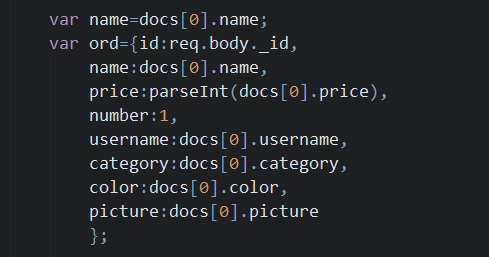
\includegraphics[scale=0.5]{32.png}
	\caption{Shopping Cart table}
	\label{fig:11 cubed graph}
\end{figure}
\\
\subsection{DB:webSite-app}
Collections:sessions\\
This Database used to store Session data which can check login, realize shopping cart.see table \ref{fig:10 cubed graph} below:
\\
\begin{figure}[h]
	\centering
	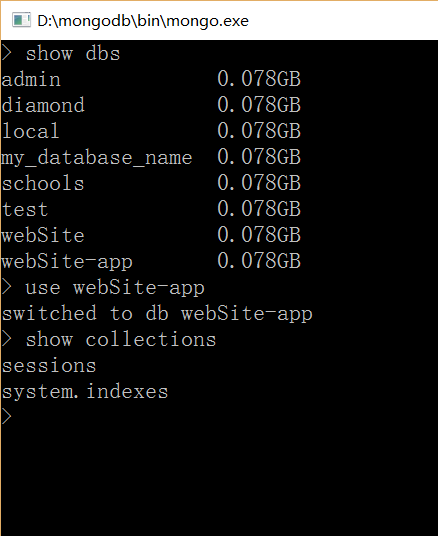
\includegraphics[scale=0.5]{31.png}
	\caption{Session}
	\label{fig:10 cubed graph}
\end{figure}
\\
\subsection{webSite : Orders}
\\
This collection used to store all orders generated from website.
see table \ref{tab:4}
\\
\begin{table}[h]
	\centering
	\begin{tabular}{l | l}
		Property & Type \\
		\hline
		userid & Number \\
		username & String\\
		itemid & Array\\
		name & Array\\
		Address & String\\
		createTime & String\\
		total & Number
	\end{tabular}
	\caption{Users table}
	\label{tab:4}
\end{table}
\\
\subsection{Code-create tables}
\\
(1)Items Table\\
See graph \ref{fig:12 cubed graph}:\\
\begin{figure}[h]
	\centering
	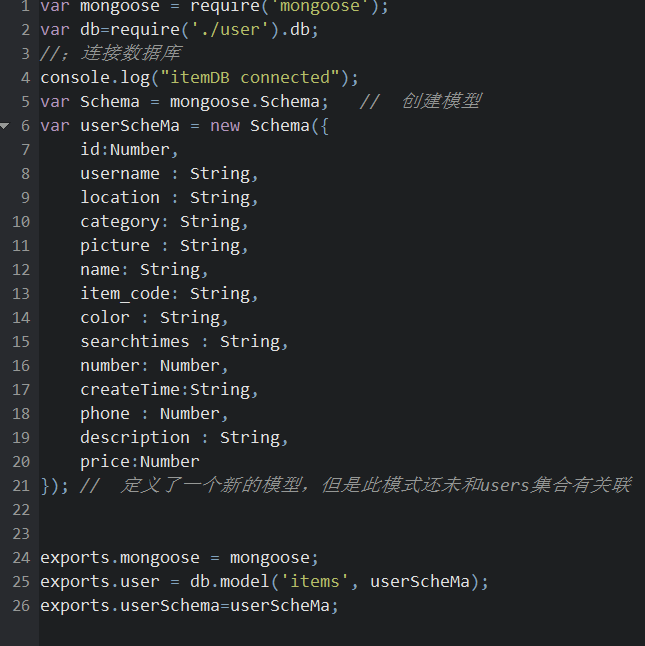
\includegraphics[scale=0.3]{33.png}
	\caption{Create Items code}
	\label{fig:12 cubed graph}
\end{figure}
\\
(2)Users Table\\
See graph \ref{fig:13 cubed graph}:\\
\begin{figure}[h]
	\centering
	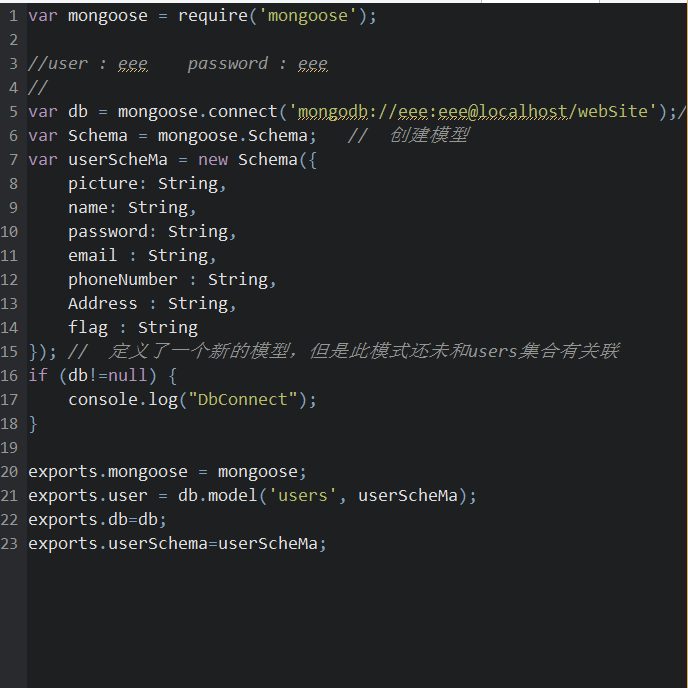
\includegraphics[scale=0.3]{34.png}
	\caption{Create User code}
	\label{fig:13 cubed graph}
\end{figure}
\\
(3)Orders Table\\
See graph \ref{fig:ord cubed graph}:\\
\begin{figure}[h]
	\centering
	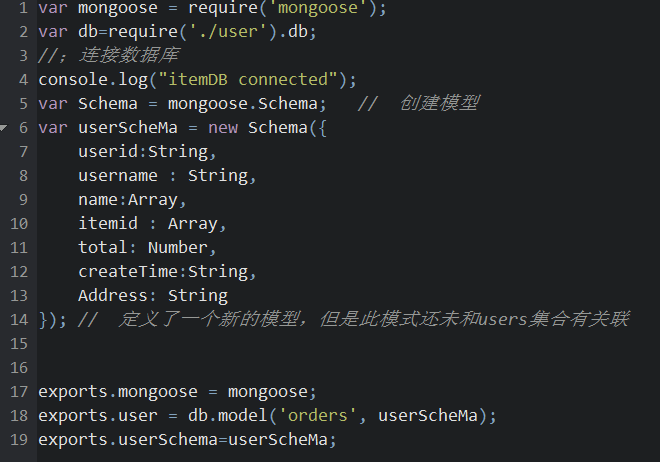
\includegraphics[scale=0.3]{54.png}
	\caption{store orders}
	\label{fig:ord cubed graph}
\end{figure}
\\
\section{Core Function}
\subsection{Hottest Item}
In the Main page of websit, the top of website have an exhibition window of rolling photographs. Every items in this window are hottest item recently, this rank list through searchtimes to decide. If there have a consumer visit a item, the searchtimes of this item will be add one.
please see graph \ref{fig:14 cubed graph}:\\   
\begin{figure}[h]
	\centering
	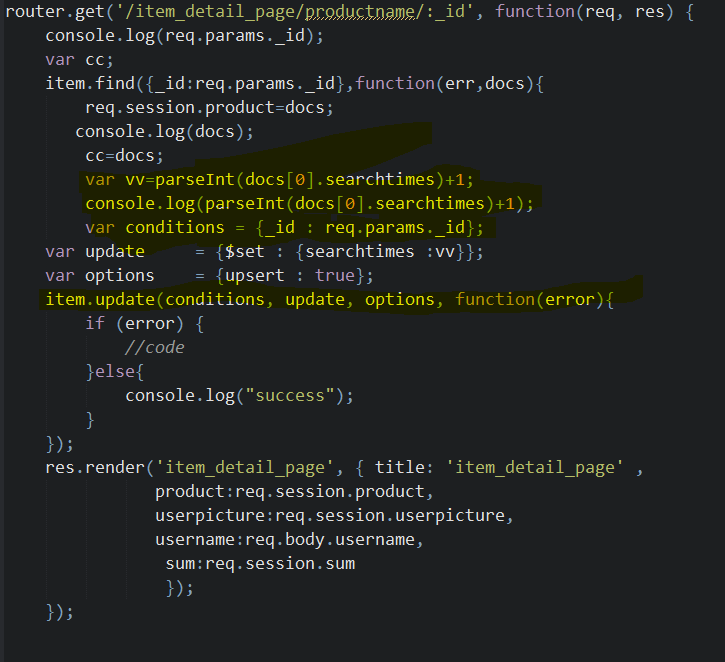
\includegraphics[scale=0.5]{35.png}
	\caption{Function searchtimes adding}
	\label{fig:14 cubed graph}
\end{figure}
\\
\subsection{Search Function}
In this website people can search item through location. It can help buyer find the nearest place to buy the product, and it can avoid fake item or long shipping time.
Search function is below :
\begin{figure}[h]
	\centering
	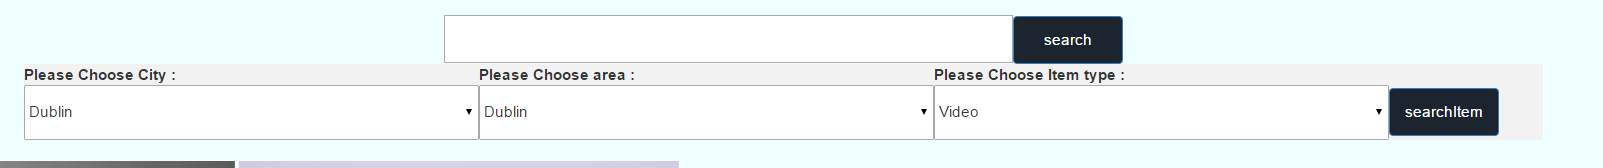
\includegraphics[scale=0.5]{36.png}
	\caption{Location Search Function}
	\label{fig:15 cubed graph}
\end{figure}
\subsection{Session}\cite{session}
This modular help project realize user keep login until user close broswer. And it more security than cookies that store request data on link.
Use Session also finish shopping cart function, when consumer add item to cart, store it on session.
see graph \ref{fig:w cubed graph},\ref{fig:f cubed graph} to check some application on website:
 \begin{figure}
 	\centering
 	\begin{subfigure}[h]{0.4\textwidth}
 		\centering
 		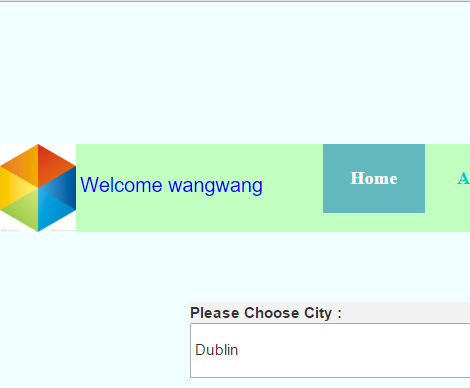
\includegraphics[width=\textwidth]{37.png}
 		\caption{Realize Login}
 		\label{fig:w cubed graph}
 	\end{subfigure}
 	\hfill
 	\begin{subfigure}[h]{0.4\textwidth}
 		\centering
 		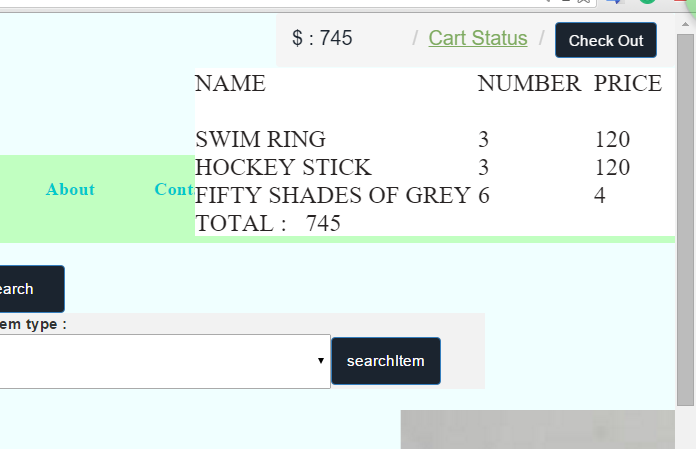
\includegraphics[width=\textwidth]{38.png}
 		\caption{Realize Shopping Cart}
 		\label{fig:f cubed graph}
 	\end{subfigure}	
 	\caption{Register page Password Check}
 	\label{fig:16 graphs}
 \end{figure}
 \\
\section{Appearance Design }
Following section will introduce my shopping website's interface design, it will be separated four parts. 
\subsection{Mainpage}
\\
This Section used to describe Main page design:\\
(1)Screen shot of main page see graph \ref{fig:18 cubed graph}: 
\\
\begin{figure}[h]
	\centering
	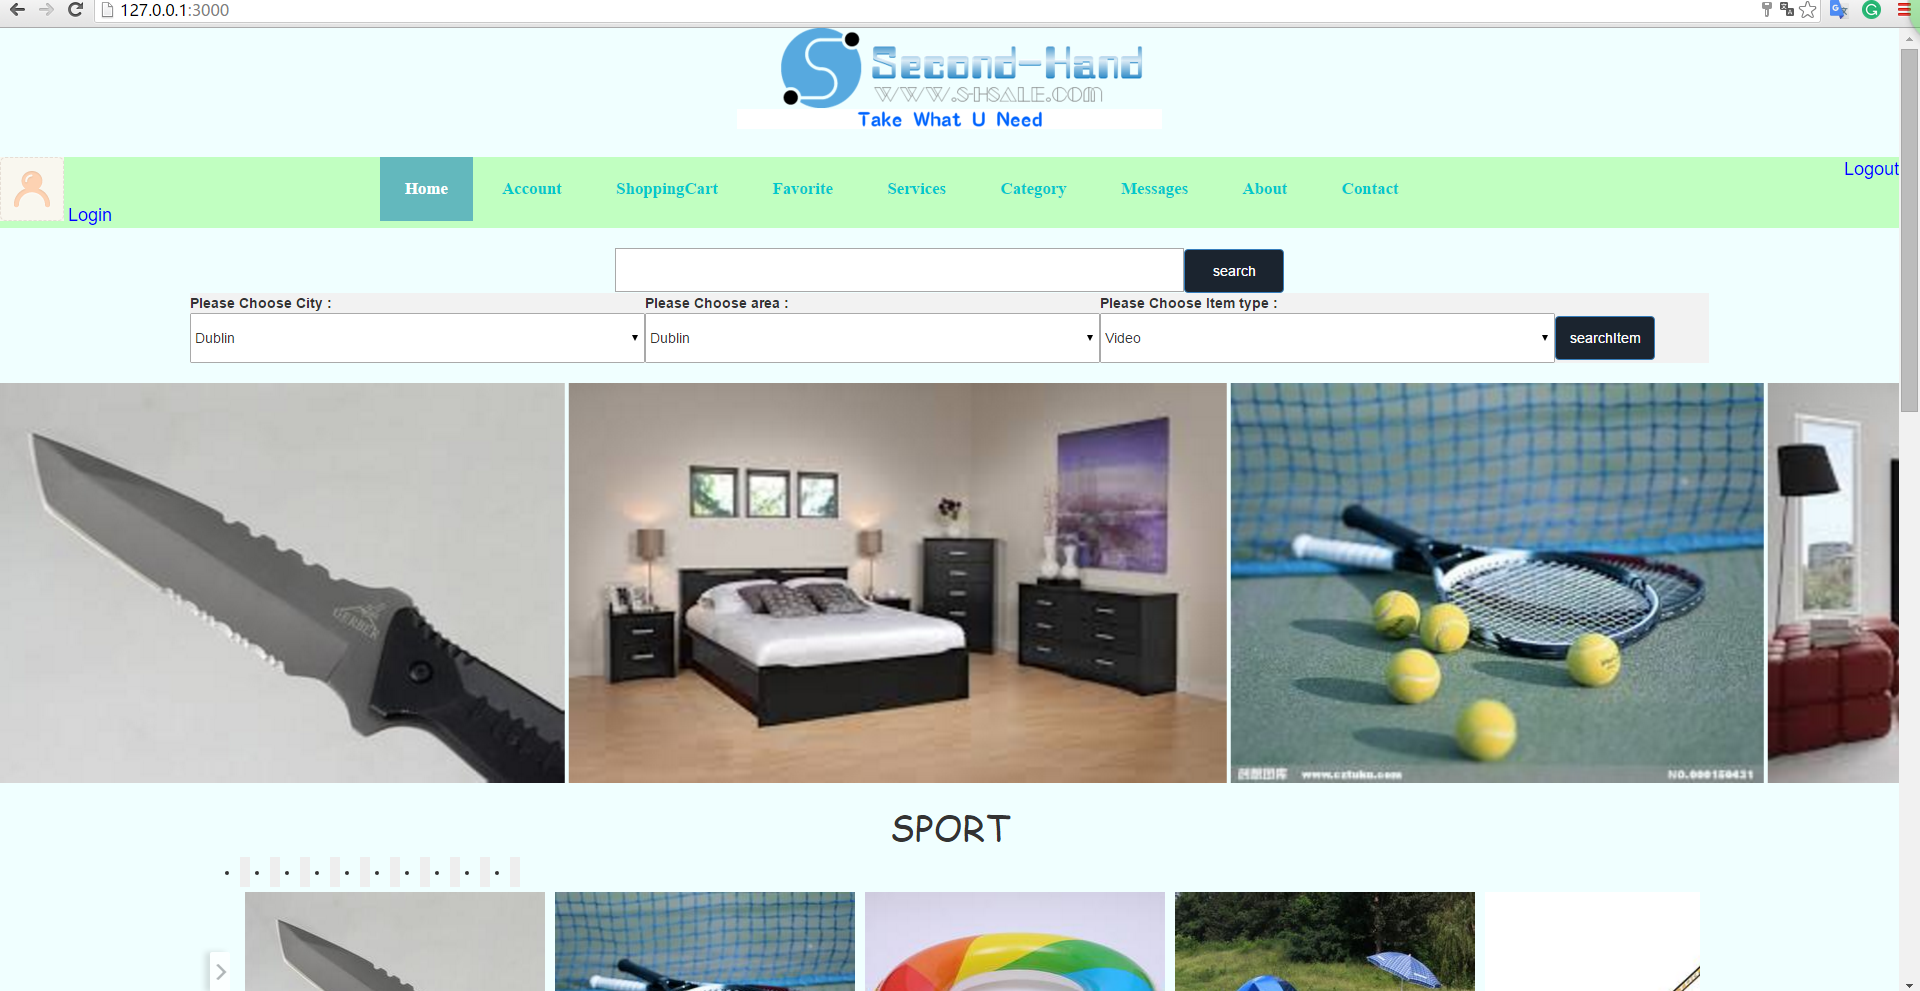
\includegraphics[scale=0.4]{21.png}
	\caption{Main-page}
	\label{fig:18 cubed graph}
\end{figure}	
\\
(2)Items Exhibition Bar see graph \ref{fig:19 cubed graph}: 
\\
In the left of Bar have two a arrow button which can switch to next page of items.\\
\begin{figure}[h]
	\centering
	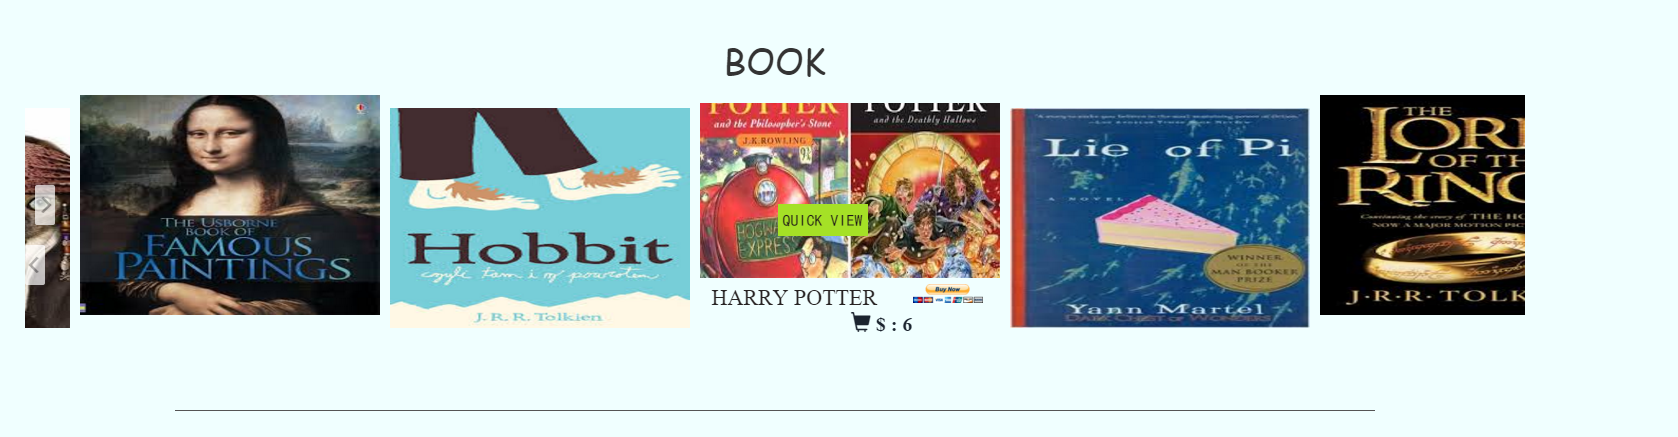
\includegraphics[scale=0.4]{40.png}
	\caption{Items Exhibition Bar }
	\label{fig:19 cubed graph}
\end{figure}	
\\
(3)Single Item View see graph \ref{fig:20 cubed graph}: 
\\
\\
1.When consumer move mouse top item will show picture like this.\\
2.The green button that in the centre of graph, when it be pressed will jump to item\_detail page.\\
3.In the bottle of graph is the name and price of product, and there also have a 
Pay-Pal Buy-Now Button help client to quick shopping.\\
\begin{figure}[h]
	\centering
	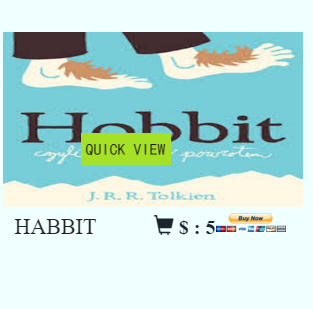
\includegraphics[scale=0.4]{41.png}
	\caption{Single-item}
	\label{fig:20 cubed graph}
\end{figure}	
\\
\subsection{User Management Page}
\\
(1)Login Page see graph \ref{fig:21 cubed graph}
\\
\begin{figure}[h]
	\centering
	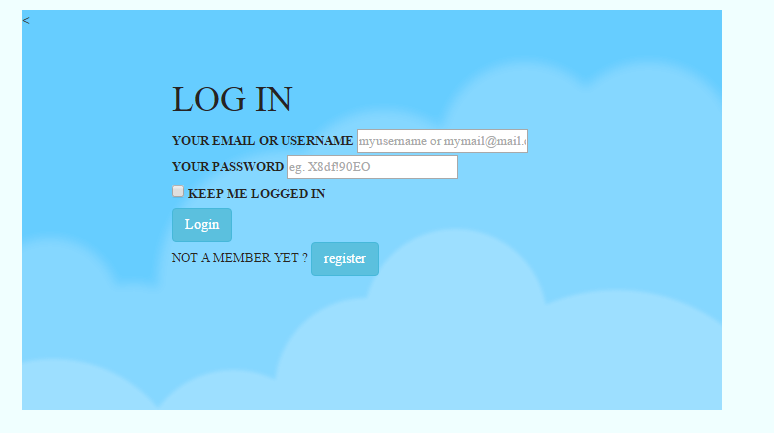
\includegraphics[scale=0.5]{22.png}
	\caption{Login}
	\label{fig:21 cubed graph}
\end{figure}
\\
(2)Register Page see graph \ref{fig:22 cubed graph}
This page require consumer fill table to register an account for shopping website.\\
\begin{figure}[h]
	\centering
	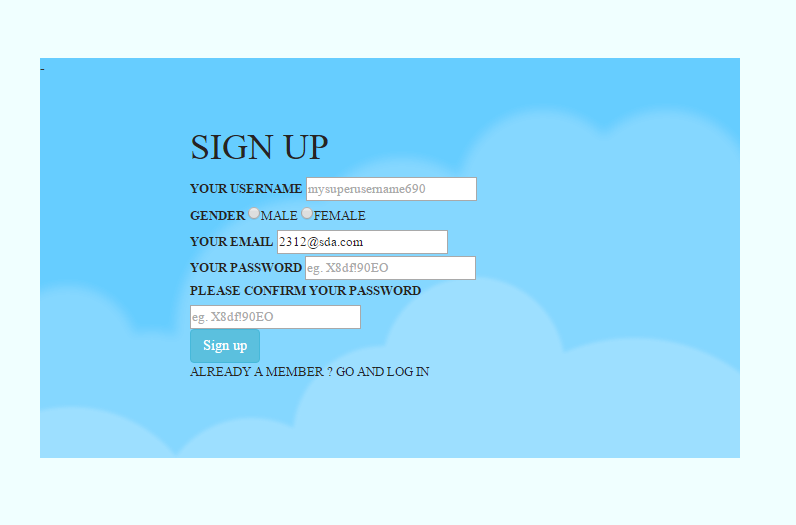
\includegraphics[scale=0.5]{42.png}
	\caption{Register}
	\label{fig:22 cubed graph}
\end{figure}
\\
(3)User Information Page see graph \ref{fig:23 cubed graph}:
\\ 
In the left of graph have 5 links which can realize different functions such as update personal information, sell product and manage selling product.\\ 
\begin{figure}[h]
	\centering
	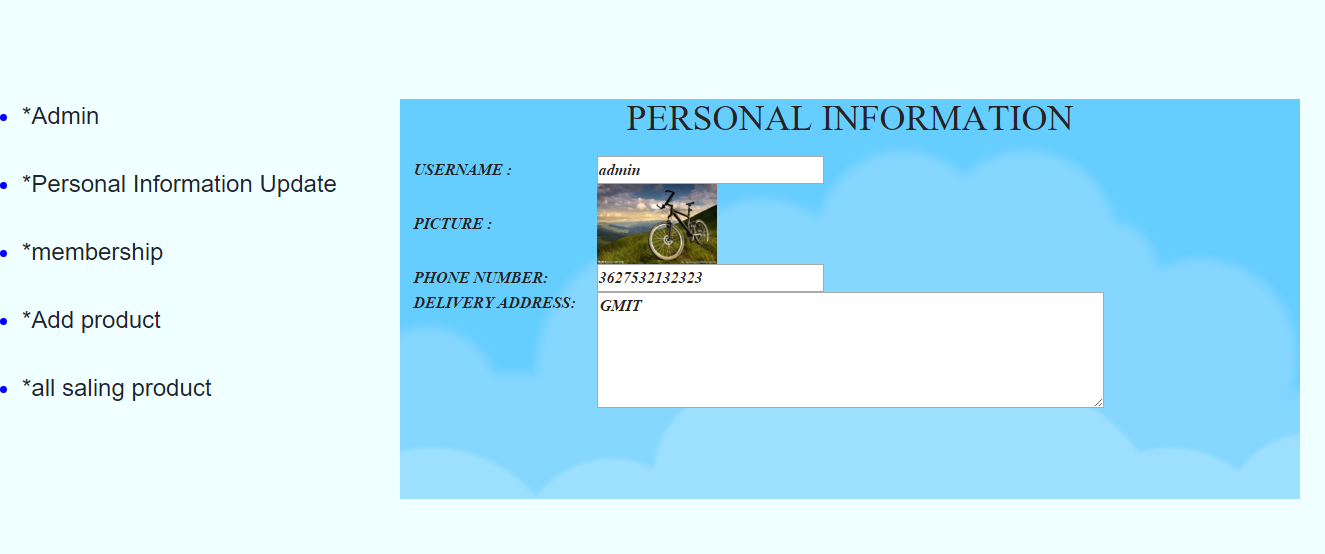
\includegraphics[scale=0.3]{43.png}
	\caption{User Information Page}
	\label{fig:23 cubed graph}
\end{figure}
\\
(4)Information update Page see graph \ref{fig:24 cubed graph}:
\\
Clients can Change his personal information such as Picture, Phone Number, Address.\\ 
 \begin{figure}[h]
 	\centering
 	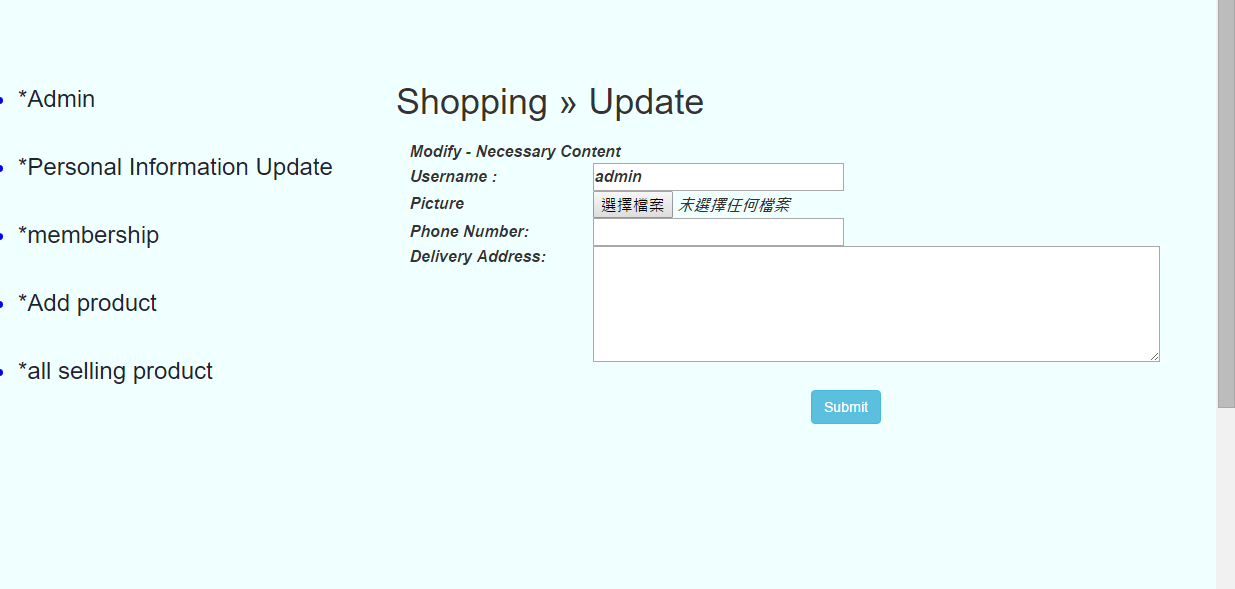
\includegraphics[scale=0.3]{44.png}
 	\caption{Information update Page}
 	\label{fig:24 cubed graph}
 \end{figure}
 \\
(5)All Orders see graph \ref{fig:ooo cubed graph}:
\\ 
\begin{figure}[h]
	\centering
	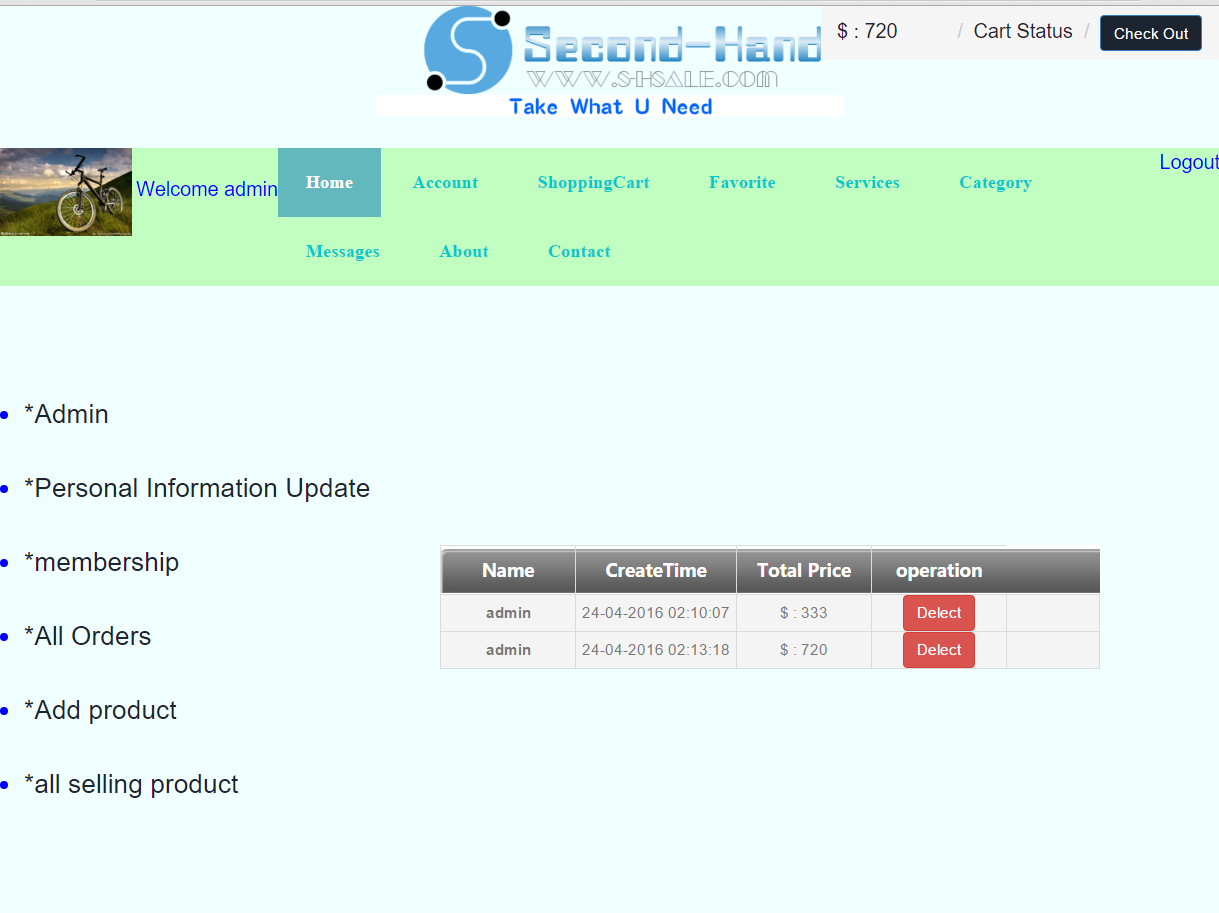
\includegraphics[scale=0.3]{53.png}
	\caption{All orders Page}
	\label{fig:ooo cubed graph}
\end{figure}
\\
(6)Admin Page see graph \ref{fig:27 cubed graph}:
\\
Admin Page only allow access by Administrator which usename is "admin" and password is "admin".\\
Administrator can update and delect users in website.\\ 
\\
In new version, people can not use same email to register a new account.
  \begin{figure}[h]
  	\centering
  	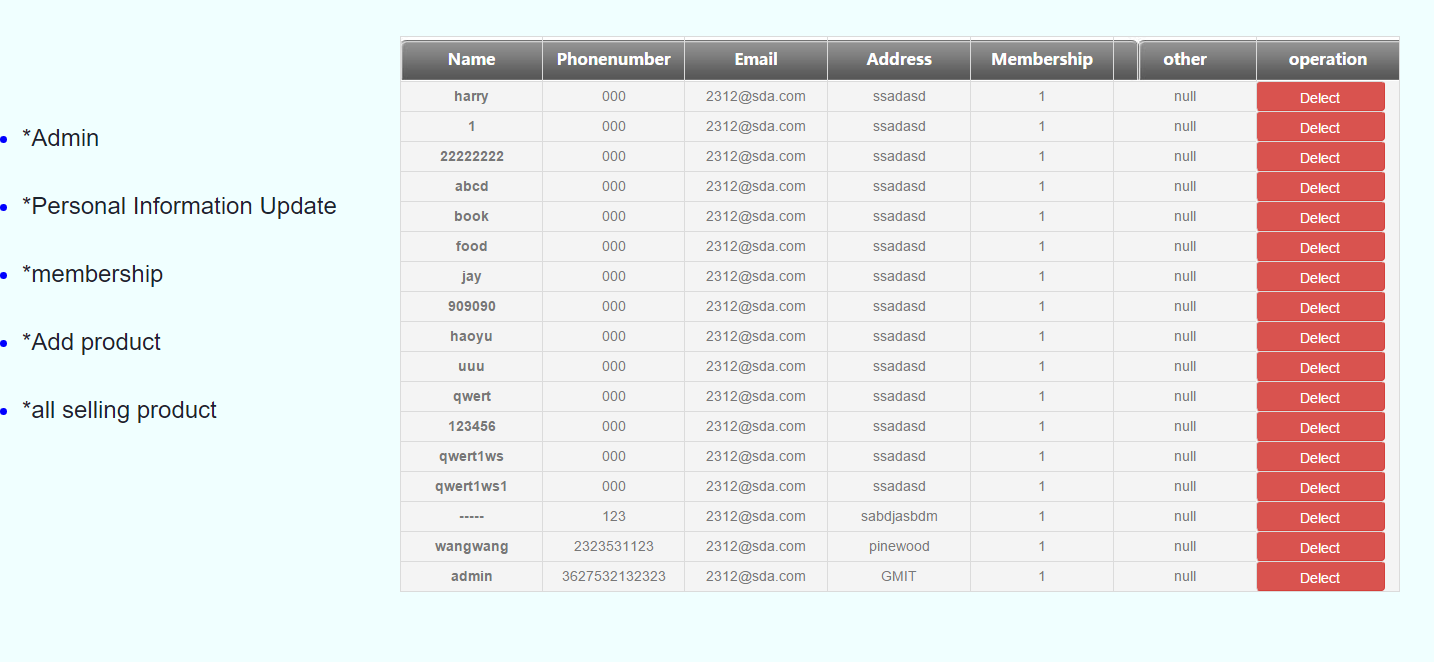
\includegraphics[scale=0.3]{47.png}
  	\caption{Selling Products Management}
  	\label{fig:27 cubed graph}
  \end{figure}
\\
\subsection{Items Page}
\\
(1)Add Product that you want to sale see graph \ref{fig:25 cubed graph}:
\begin{figure}[h]
	\centering
	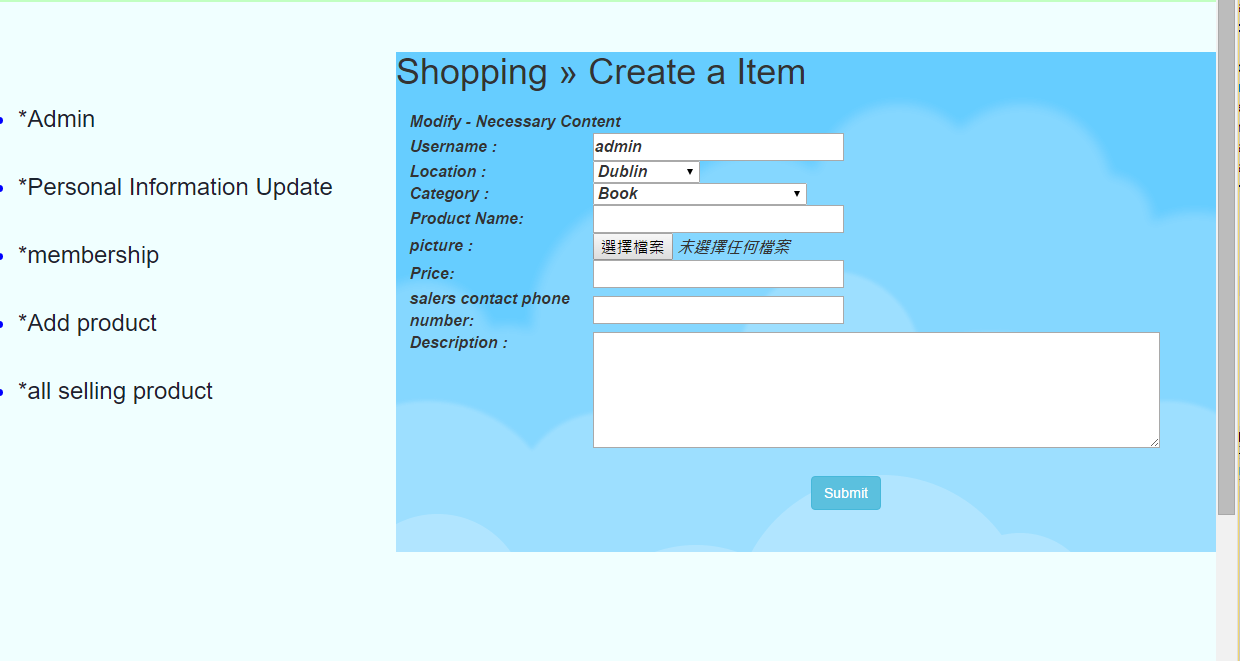
\includegraphics[scale=0.3]{45.png}
	\caption{Add Selling Products}
	\label{fig:25 cubed graph}
\end{figure}
\\
(2)Selling Products Management see graph \ref{fig:26 cubed graph}:
This Page below show all items that be created by consumers. Include some details such as name, price, createTime.\\
\begin{figure}[h]
	\centering
	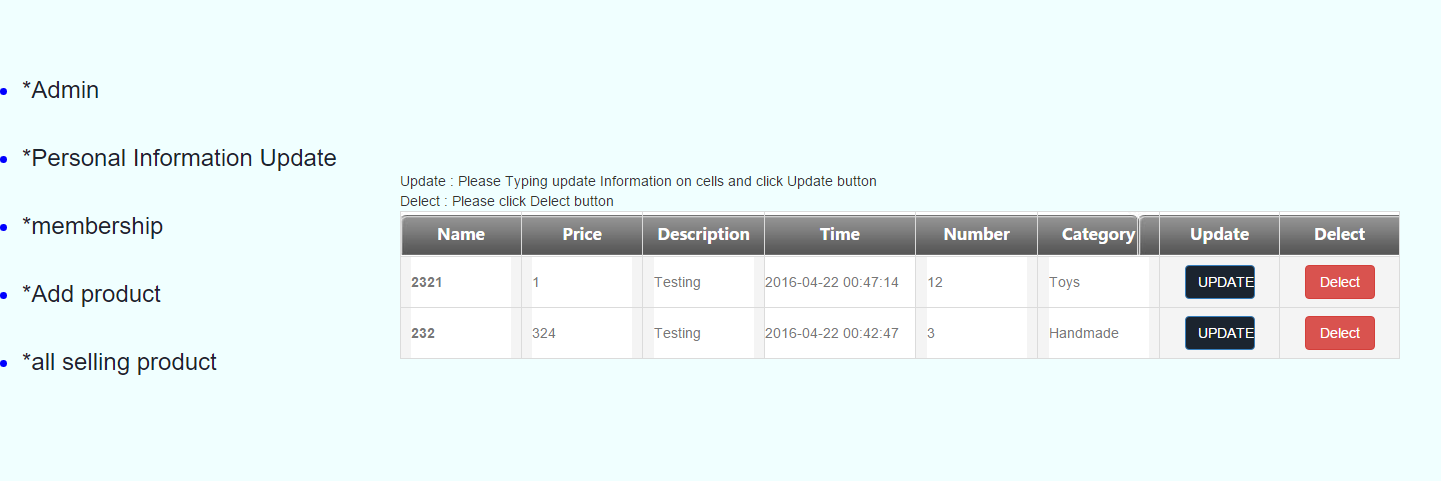
\includegraphics[scale=0.3]{46.png}
	\caption{Selling Products Management}
	\label{fig:26 cubed graph}
\end{figure}
\\
(3)Items Detail Page see graph \ref{fig:28 cubed graph}:
In the bottle of Graph is an area offer consumer write down them felling and feedback about this product.\\ 
\begin{figure}[h]
	\centering
	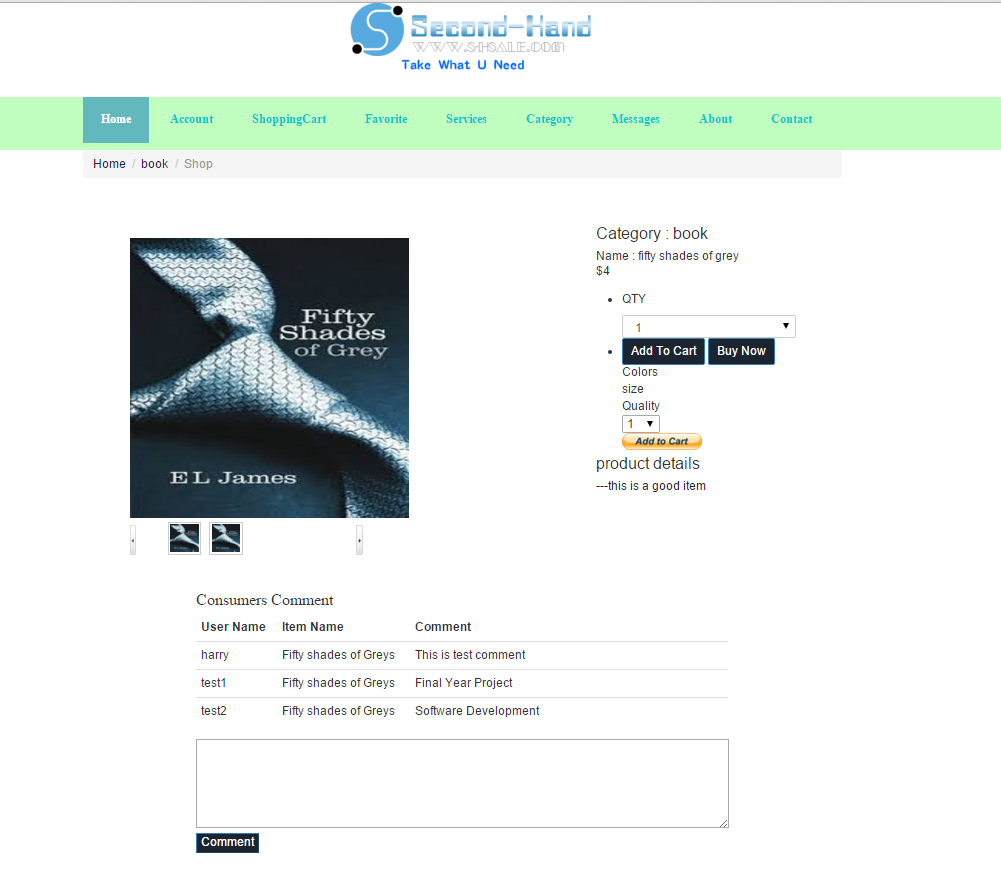
\includegraphics[scale=0.3]{48.png}
	\caption{Item Detail Page}
	\label{fig:28 cubed graph}
\end{figure}
\\
(4)OrderCheck Page see graph \ref{fig:29 cubed graph}:
Fist area is to set delivery address.\\
Second is check and confirm order is or not correct.\\
Then click PayNow button.\\
\begin{figure}[h]
	\centering
	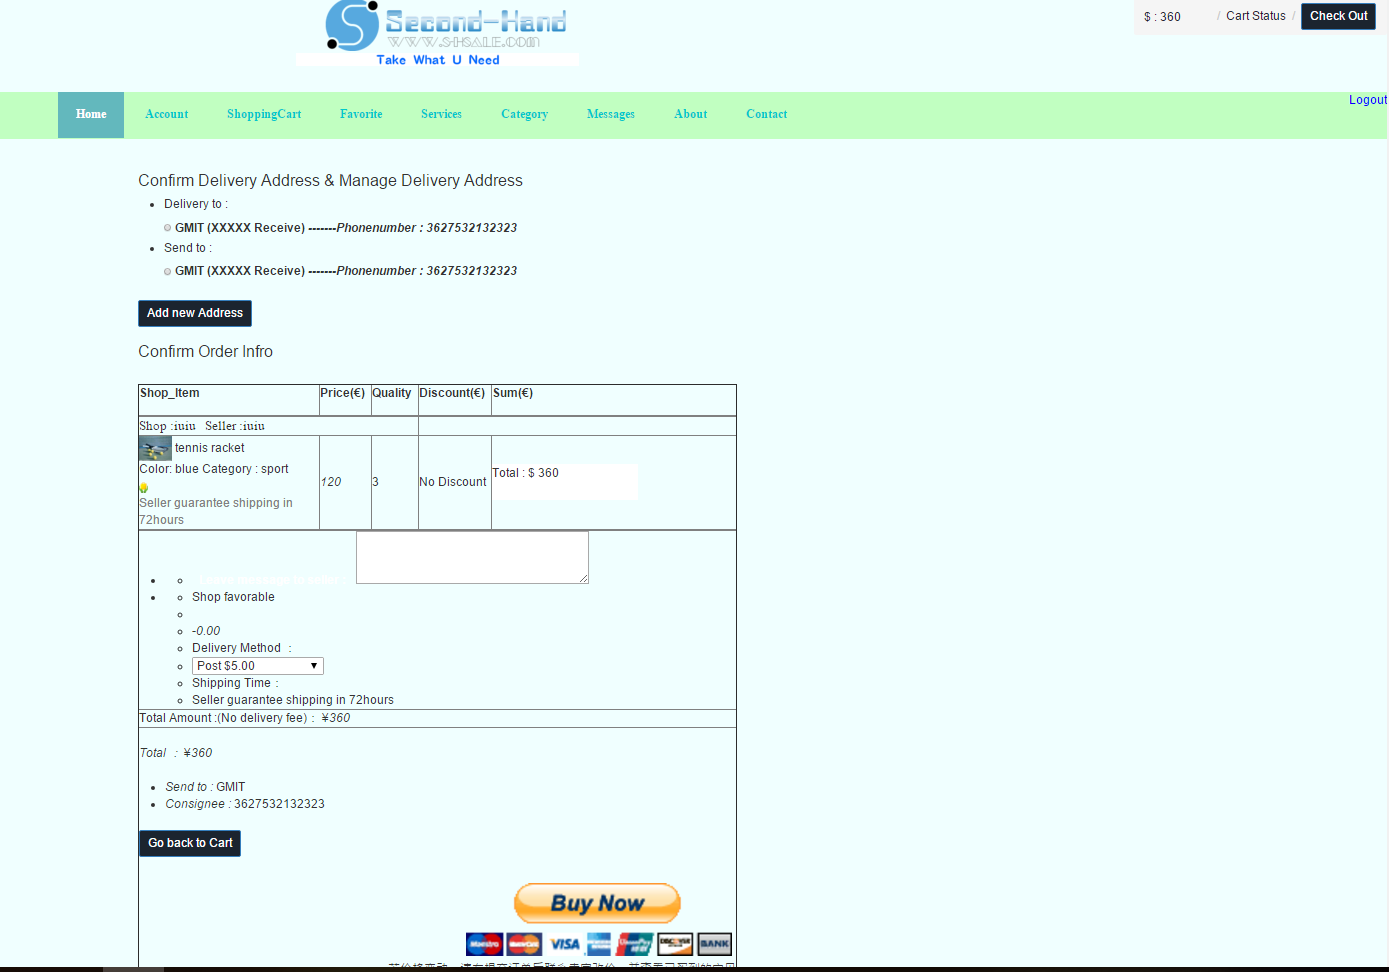
\includegraphics[scale=0.3]{49.png}
	\caption{OrderCheck Page}
	\label{fig:29 cubed graph}
\end{figure}
\\
(5)Search Page see graph \ref{fig:30 cubed graph}:
All products will be ranked by search times.\\
\begin{figure}[h]
	\centering
	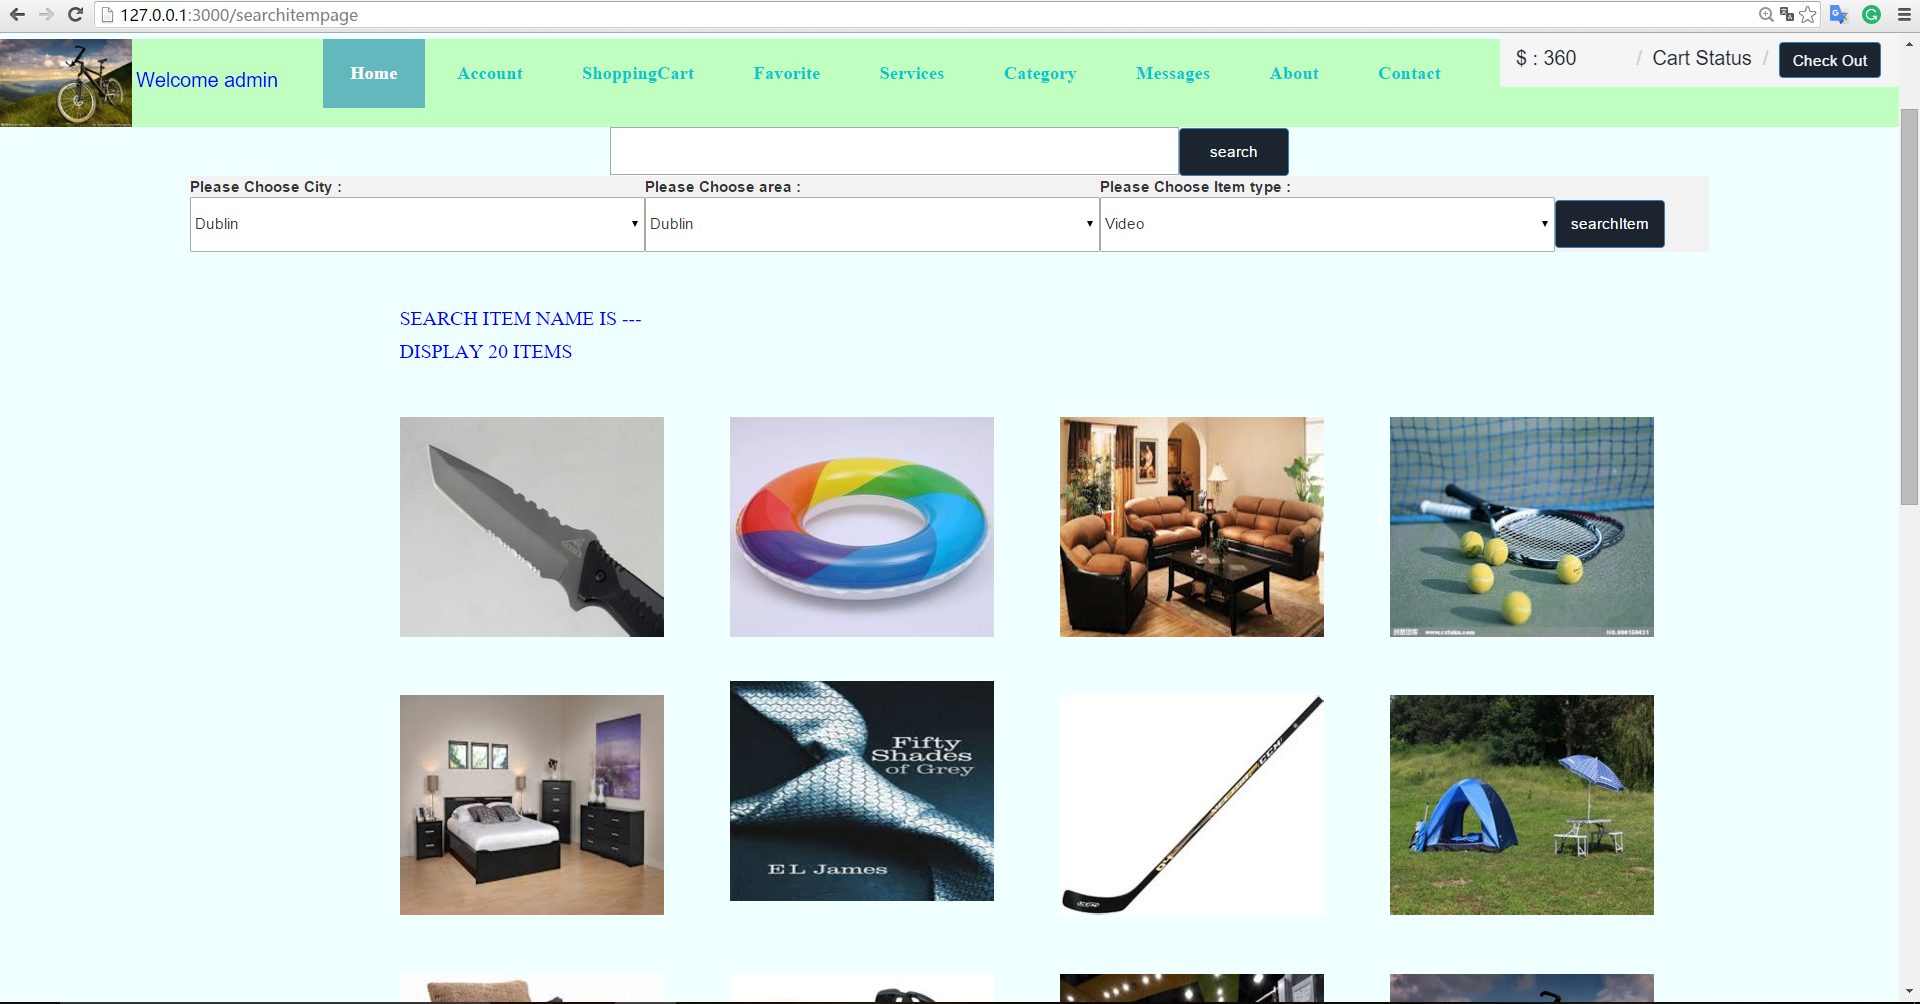
\includegraphics[scale=0.3]{50.png}
	\caption{Search Page}
	\label{fig:30 cubed graph}
\end{figure}
\\
(6)Shopping Cart see graph \ref{fig:31 cubed graph}:
\\
\begin{figure}[h]
	\centering
	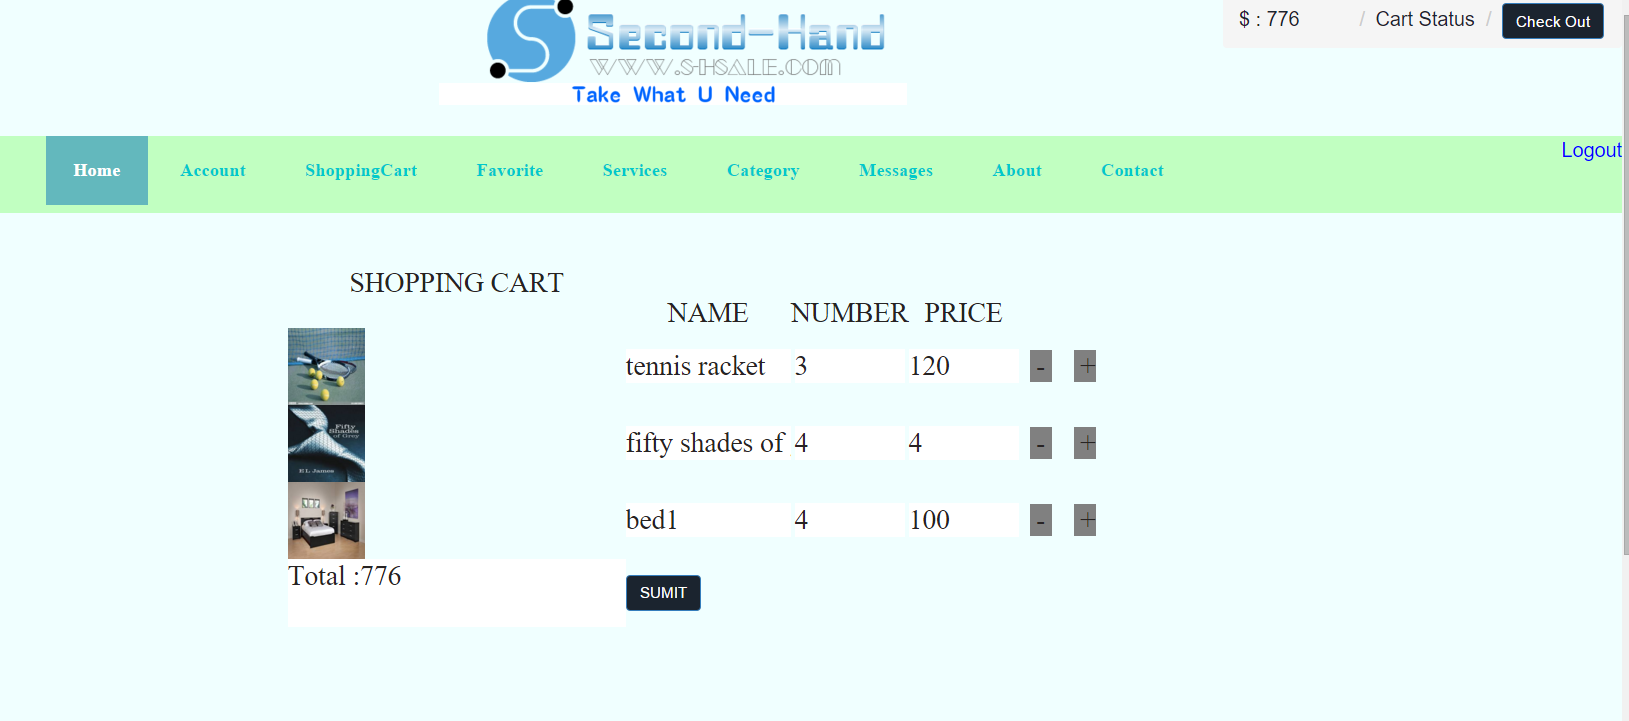
\includegraphics[scale=0.4]{51.png}
	\caption{Shopping Cart}
	\label{fig:31 cubed graph}
\end{figure}
\\
(7)Shopping Cary Mini State window see graph \ref{fig:32 cubed graph}:
\\
\\
When consumers put mouse top Cart State will show this.\\
\begin{figure}[h]
	\centering
	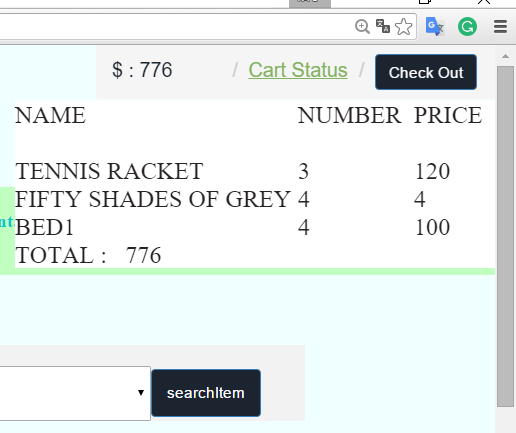
\includegraphics[scale=0.5]{52.png}
	\caption{Shopping Cary Mini State window}
	\label{fig:32 cubed graph}
\end{figure}
\\